\documentclass[12pt,a4paper]{article}
\usepackage[utf8]{inputenc}
\usepackage[spanish]{babel}
\usepackage{amsmath}
\usepackage{amsfonts}
\usepackage{amssymb}
\usepackage{makeidx}
\usepackage{graphicx}
\usepackage[left=2cm,right=2cm,top=2cm,bottom=2cm]{geometry}

\author{Felipe Alvarado Galicia}
\title{DENAVIT-HARTENBERG}
\date{Profesor:Carlos Enrique Moran Garabito\\
Materia: Cinematica de Robots\\
17 de septiembre de 2019}

\begin{document}
\maketitle
 
\includegraphics[scale=1]{logo1.png}\\
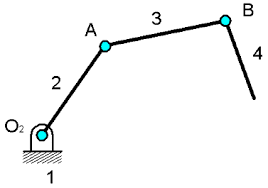
\includegraphics[scale=1]{imag5.png} 
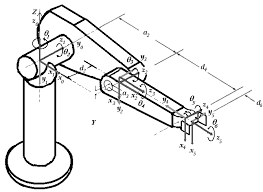
\includegraphics[scale=1]{imag8.png}\\\\\\\\\\\\\\\\\\\\\\\\\\\\\\\\\\\\\\\\\\\\\\

\tableofcontents

\section{La representación Denavit-Hartenberg
}
Se trata de un procedimieto sistemático para describir la estructura cinemática de una cadena articulada constituida por articulaciones con. un solo grado de libertad.\\
 Para ello, a cada articulación se le asigna un Sistema de Referencia Local con origen en un punto i Q y ejes ortonormales { } , , i i i X Y Z , comenzando con un primer S.R fijo e inmóvil dado por los ejes { } 0 0 0 , , X Y Z , anclado a un punto fijo 0 Q  de la Base sobre la que está montada toda la estructura de la cadena.\\
Este Sistema de Referencia no tiene por qué ser el Universal con origen en (0,0,0) y la Base canónica.
\subsection{Asignación de Sistemas de Referencia}
Las articulaciones se numeran desde 1 hasta n. A la articulación i -esima se le asocia su propio eje de rotación como Eje Z i-1, de forma que el eje de giro de la 1ª articulación es Zo de forma que el eje de giro de la 1ª articulación es n-esima articulación, Zn-1.\\
En la Figura adjunta se muestra la estructura del Robot PUMA junto con sus articulaciones y ejes de rotación.\\
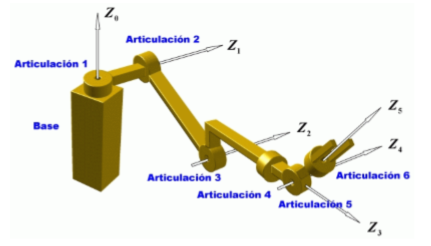
\includegraphics[scale=1]{2.PNG} \\
Para la articulación i-ésima (que es la que gira alrededor de Zi-1), la elección del origen de coordenadas Qi y del eje Xi sigue reglas muy precisas en función de la geometría de los brazos articulados. el eje Yi por su parte, se escoge para que el sistema {Xi, Yi, Zi} sea dextrógiro. \\
La especificación de cada eje Xi depende de la relación espacial entre Zi y Zi-1, distinguiéndose 2 casos:\\
\subsubsection{Zi y Zi-1  no son paralelos}
Entonces existe una única recta perpendicular a ambos, cuya intersección con los ejes proporciona su mínima distancia (que puede ser 0). Esta distancia, ai,  medida desde el eje Zi-1 hacia el eje Zi (con su signo), es uno de los parámetros asociados a la articulación i-ésima.\\
La distancia di desde Qi-1 a la intersección de la perpendicular común entre Zi-1 y Zi con Zi-1 es el 2º de los parámetros. En este caso, el eje Xi es esta recta, siendo el sentido positivo el que va desde el eje Zi-1 al Zi si ai>0. El origen de coordenadas Qi es la intersección de dicha recta con el Eje Zi.\\
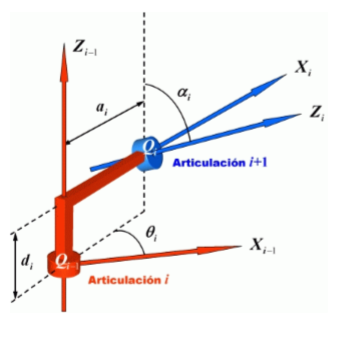
\includegraphics[scale=1]{3.PNG} \\
\subsubsection{Zi y Zi-1  son paralelos}
En esta situación el Eje Xi se toma en el plano conteniendo a Zi y Zi-1 y perpendicular a ambos.\\
El origen Qi es cualquier punto conveniente del eje Zi.\\
El parámetro ai es, como antes, la distancia perpendicular entre los ejes Zi y Zi-1, y di es la distancia desde Qi-1.\\
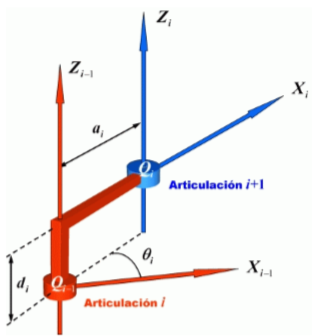
\includegraphics[scale=1]{4.PNG} \\
Una vez determinado el eje Xi, a la articulación i-ésima se le asocia un 3er parámetro fijo ai que es el ángulo que forman los ejes Zi y Zi-1 en relación al eje Xi.\\
Nótese que cuando el brazo i-ésimo (que une rígidamente las articulaciones i e i+1) gira en torno al eje Zi-1 (que es el de rotación de la articulación i), los parámetros ai, di y ai permanecen constantes, pues dependen exclusivamente de las posiciones/orientaciones relativas entre los ejes Zi-1 y Zi, que son invariables. Por tanto, ai, di y ai pueden calcularse a partir de cualquier configuración de la estructura articulada, en particular a partir de una configuración inicial estándar. Precisamente el ángulo 0i de giro que forman los ejes Xi-1 y Xi con respecto al eje Zi-1 es el 4º parámetro asociado a la articulación i y el único de ellos que varía cuando el brazo i gira.
Es importante observar que el conjunto de los 4 parámetros ai, di y ai y
 determina totalmente el Sistema 
de Referencia de la articulación i+1 en función del S.R de la articulación i.





\section{ALGORITMO}
\subsection{paso 0}
Determinar el número de eslabones y el número de articulaciones. En nuestro caso se tiene que el número de eslabones es n+1, con n=7 y el número de articulaciones es n; por lo tanto hay 8 eslabones en este ejemplo. Para los eslabones, la numeración comienza en 0, el eslabón 0 es la base y el eslabón n=7 es el efector final. Las articulaciones comienzan a numerarse en 1.\\
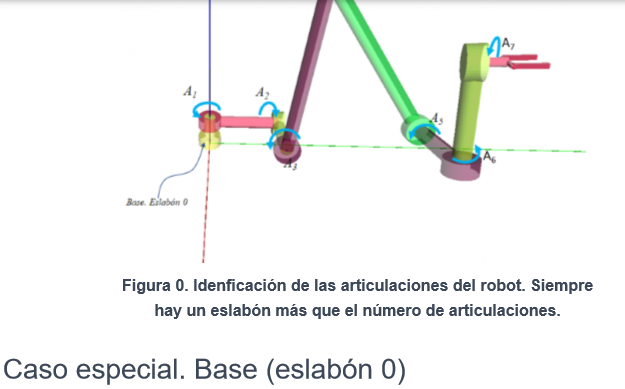
\includegraphics[scale=1]{1.PNG} \\
Determinar la dirección del eje Zo.\\
El eje Zo se escoge de tal forma que este alineado (es decir además de paralelo debe estar en la misma línea) con el eje de la articulación A1 (figura 3),  el origen del sistema de referencia Bo (base) se sitúa en cualquier punto del eje Zo.\\
Los ejes  , ,   del sistema de referencia  situado en el eslabón   (base) son fijos (no rotan), se escogen de tal manera que sea un sistema que obedece a la regla de la mano derecha 
\subsection{paso 1}
Para cada eslabón  i=1,2,3…n-1 ( en este ejemplo n-1=6, el i=0 es la base y para el efector final i=7, véase paso 0)  hay tres pasos a realizar para elegir la dirección  y la dirección , con ello el eje  se elige simplemente de tal forma que el sistema de referencia  sea un sistema que obedece a la regla de la mano derecha (dextrógiro).\\
Determinar la dirección de los ejes zi con i=1,2,3…n-1.\\
El eje zi se escoge de tal forma que esté alineado (en la misma línea) con el eje de la articulación Ai+1.\\
Cada eje zi está montado sobre el eslabón i.\\
Para el eslabón 1, según el robot SSRMS de ejemplo en estudio, a continuación se muestra la configuración del eslabón 1 con el eslabón 2, aún sin representar el eje zi.\\
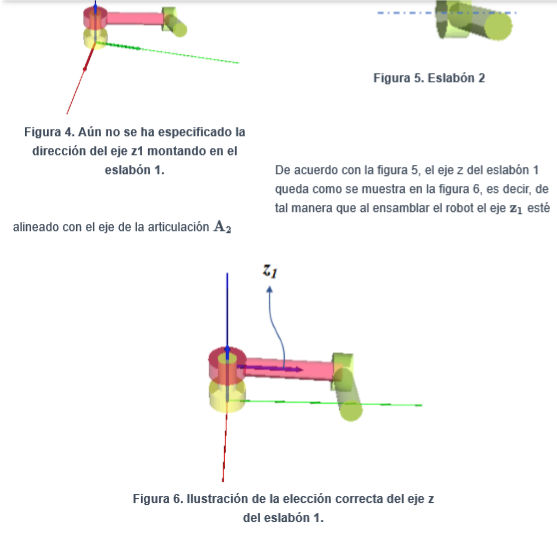
\includegraphics[scale=1]{5.PNG} \\
\subsection{Paso 2}
Determinar la dirección de los ejes xi con i=1,2,3…n-1.\\ Caso 1.
Si los ejes zi y zi-1 se intersecan , la dirección del eje xi esta dada por la dirección del vector xi=zi*zi-1.\\
Para el caso 1, donde ocurre tal intersección se coloca el origen del sistema de referencia Bi.
De la figura 8, observe que este caso se cumple para los ejes xi con i=1,2,5,n-1.\\
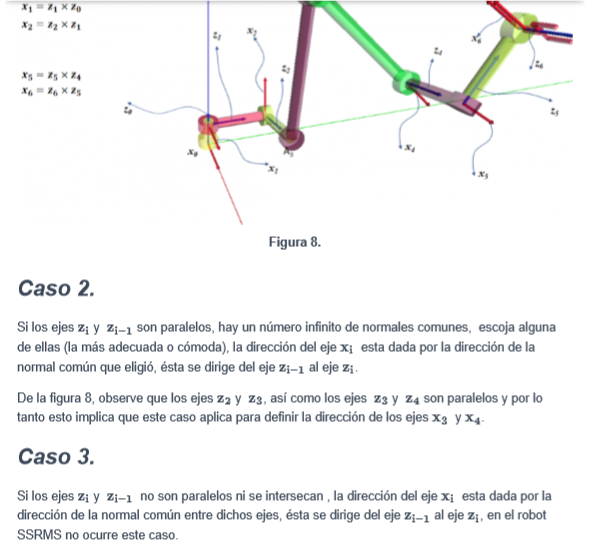
\includegraphics[scale=1]{7.PNG} \\
\paragraph{binliografia}
file:///C:/Users/acer/Documents/7mo%20Cinematica%20de%20robots/Robótica_%20Algoritmo%20de%20Denavit–Hartenberg.%20Caso%20de%20estudio%20SSRMS%20–%20Mafer's%20Tech%20Holdings%20industries.pdf \\

\end{document}